
\documentclass[preprint,12pt]{elsarticle}

\usepackage[spanish]{babel}
\usepackage{amssymb}
\usepackage{graphicx}
\usepackage{lineno}
\usepackage[utf8]{inputenc}
\usepackage{url}
\usepackage{natbib}

\begin{document}
	
	\begin{frontmatter}

		\title{\huge  Comparativa de Cuadro de Mando Integral (BSC) y Modelo de Negocio Canvas (BMC) }
		\author{Robles Flores, Anthony Richard	                (2016056192)}
		\author{Estrella Palacios, Katherine Lizbeth			(2015050948)}
		\author{Sosa Bedoya, Sharon Fiorela				(2016054460)}
		\author{Torres Beltran , Johanna Andrea			(2020067849)}
		\address{Tacna, Perú}
		


%%INICIO abstract
\begin{abstract}
The Balanced Scorecard (CMI Spanish Acronym) and the Canvas model can be linked as complementary tools for entrepreneurs. The first develops goals and operational measures in four main perspectives for the purpose of achieving the mission and strategy. The second suggest a (re-) evolution in generating business models, establishing nine sections that reflect their logic. In the article a working model is developed that, based on the need for a CMI it relates its design to the information previously collected in the Canvas model, pointing their mutual necessity
\end{abstract}
%%FIN abstract


\end{frontmatter}

%%INICIO Resumen
\section{Resumen}
El Cuadro de Mando Integral (BSC) y el modelo Canvas pueden enlazarse como herramientas complementarias para los emprendedores. La primera desarrolla objetivos y medidas operativas en cuatro perspectivas principales para alcanzar la misión y estrategia. La segunda ha supuesto una (re-)evolución en la generación de modelos de negocio, estableciendo nueve apartados que reflejan su lógica. En el artículo se desarrolla un modelo de trabajo que, partiendo de la necesidad de disponer de un BSC, relaciona su diseño con la información recogida previamente en el modelo Canvas, señalando su mutua necesidad.
%%FIN Resumen


%%INICIO Introducción
\section{Introducción}
En la literatura de dirección estratégica, el cuadro de mando integral (Balanced Scorecard, BSC de aquí en adelante) se considera como una de las herramientas más conocidas e importantes para la implementación de la estrategia. Su utilidad destaca en el momento de desarrollar objetivos operativos para la comunicación de la misión y estrategia de la empresa, así como en la medición del grado de consecución de éstas, proponiendo convertir la estrategia en un conjunto de medidas de actuación que permiten su traducción y gestión. De esta forma, un BSC ha de estar constituido por un conjunto limitado de medidas financieras y no financieras organizadas en cuatro principales perspectivas interrelacionadas entre sí (Da Silva et al., 2013), que describen la estrategia organizativa a través de relaciones causa-efecto entre los indicadores: (1) financiera, (2) cliente, (3) interna e (4) innovación y crecimiento.\\ \\
Canvas es una herramienta para la generación de modelos de negocios desarrollado por Alex Osterwalder (2004), que permite trabajar sobre la base de cómo una organización crea, proporciona y captura valor. Como indican Zott et al., (2011), aunque no hay consenso entre los académicos sobre lo que es un modelo de negocio, este concepto sí incluye una visión holística del negocio como unidad de análisis donde se enfatiza el papel de las actividades de la empresa en la generación de valor. Especialmente adecuado en la fase start-up o de búsqueda del modelo de negocio, en la que predominan la alta complejidad y la dificultad de considerar numerosas variables, el Canvas propone un lenguaje y visualización que permite describirlo fácilmente, facilitando su evolución y adaptación, de forma intuitiva, siendo fácil de usar y comprender para definir la alternativa estratégica seleccionada por la nueva empresa, donde exista una propuesta de valor que recoja, además de la importancia de los procesos internos, la relevancia de las relaciones con los diferentes stakeholders.



%%FIN Introducción


%%INICIO Marco Teórico
\section{Marco Teórico}

%%----------------------------------------------------------------------------------------------------------------------------------------------------------
	\subsection{\textbf{Cuadro de Mando Integral (BSC)}}
	
xxxxxxxxxxxxxxxxxxxxxxxxxxxxxxxxxxxxxxxxxxxxxxxxxxxxxxxxxxxxxxxxxxxxxxxxxxxxxxxxxxxxxxxxxxx\cite{referenciarobles1}

\subsubsection{\textbf{Subtitulo 1}}

	\begin{itemize}
	\item a
	\item b
	\item c
	\end{itemize}



\subsubsection{\textbf{Subtitulo 2}}

	\begin{itemize}
	\item a
	\item b
	\item c
	\end{itemize}

%%----------------------------------------------------------------------------------------------------------------------------------------------------------

	\subsection{\textbf{Modelo de Negocio Canvas (BMC) }}
	
xxxxxxxxxxxxxxxxxxxxxxxxxxxxxxxxxxxxxxxxxxxxxxxxxxxxxxxxxxxxxxxxxxxxxxxxxxxxxxxxxxxxxxxxxxxxxxxxxxxxxxxxxxxx

	\subsubsection{\textbf{Subtitulo 1}}
	\begin{itemize}
	\item{\textbf{1. Punto1: }}XXXXXXXXXXXXX
	\item {\textbf{2. Punto2: }}XXXXXXXXXXXX
	\item {\textbf{3. Punto3: }}XXXXXXXXXXXX
	\end{itemize}

	\subsubsection{\textbf{Subtitulo 2}}

	\begin{itemize}
	\item a
	\item b
	\item c
	\end{itemize}

	\subsubsection{\textbf{Subtitulo 3}}

	\begin{figure}[htb]
		\begin{center}
			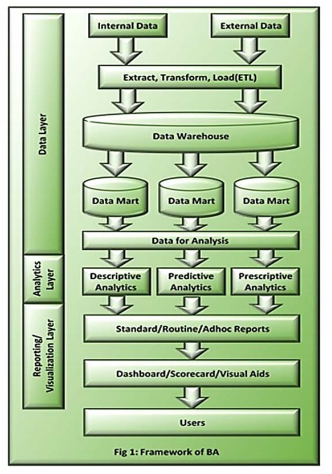
\includegraphics[height=9cm]{./IMAGENES/BAFramework} 
			\caption{Framework de BA}
		\end{center}
	\end{figure}


%%FIN Marco Teórico
%%----------------------------------------------------------------------------------------------------------------------------------------------------------


%COMPRACION

\section{Comparación entre Cuadro de Mando Integral (BSC) y Modelo de Negocio Canvas (BMC)}
A continuación se muestra la comparación entre Cuadro de Mando Integral (BSC) y Modelo de Negocio Canvas (BMC)
	
	\begin{itemize}

	\item{\textbf{1.}} XXXXXXXXXXXXXXXXXXXX
	\item{\textbf{2.}} XXXXXXXXXXXXXXXXXXXX
	\item{\textbf{3.}} XXXXXXXXXXXXXXXXXXXX
	\item{\textbf{4.}} XXXXXXXXXXXXXXXXXXXX
	\item{\textbf{5.}} XXXXXXXXXXXXXXXXXXXX
	\item{\textbf{6.}} XXXXXXXXXXXXXXXXXXXX
	\item{\textbf{7.}} XXXXXXXXXXXXXXXXXXXX
	\end{itemize}

%%----------------------------------------------------------------------------------------------------------------------------------------------------------

%CONCLUSIONES
\section{Conclusiones}

%%****
	\begin{itemize}
		\item XXXXXXXXXXXXXXXXXXXX
		\item XXXXXXXXXXXXXXXXXXXX
		\item XXXXXXXXXXXXXXXXXXXX
	\end{itemize}

%%----------------------------------------------------------------------------------------------------------------------------------------------------------

%RECOMENDACIONES
\section{Recomendaciones}	

	\begin{itemize}
		\item XXXXXXXXXXXXXXXXXXXX
		\item XXXXXXXXXXXXXXXXXXXX
		\item XXXXXXXXXXXXXXXXXXXX
	\end{itemize}


%%----------------------------------------------------------------------------------------------------------------------------------------------------------

	
	\newpage
	\bibliographystyle{apalike}
	\bibliography{BIBLIOGRAFIA}	



\end{document}

